\chapter{\babEmpat}

Bab ini memaparkan bagaimana mengimplementasikan metode yang diusulkan pada bab
sebelumnya ke dalam bentuk kode program, mengimplementasikan ide dari penelitian
ini yang dievaluasi dalam \testbed~serta hasil yang didapat dievaluasi dan
dianalisa dari percobaan yang telah dilakukan berdasarkan beberapa skenario.

% Uji Coba {{{ %
\section{Uji Coba}
Pengujian dalam penelitian ini ditujukan untuk membandingkan serta mengamati
kinerja dari sistem \tracking~metode adaptif dibandingkan dengan
\tracking~metode non-adaptif untuk setiap skenario pengujian yang telah
dipaparkan pada Bab 3. Selain itu, dijelaskan juga mengenai lingkungan uji coba
yang digunakan, meliputi topologi serta spesifikasi masing-masing perangkat.

% Lingkungan Uji Coba {{{ %
\subsection{Lingkungan Uji Coba}

Metode yang telah diusulkan dievaluasi dalam lingkungan
\testbed~(Gambar\ref{fig:testbed}) yang dibangun
sendiri. \Testbed~yang dibangun merupakan komunikasi \server~dan \client.
\Client~dibagi menjadi dua macam, yaitu: \publisher~\client~dan
\subscriber~\client. \Testbed~dibangun dalam lingkungan pemrograman \nodejs.

Sedangkan spesifikasi perangkat keras dideskripsikan sebagai berikut.
Spesifikasi pada server, \processor~Intel(R) Xeon(R) CPU E5-2630L 2.4GHz, RAM
(\ram) 512Mb, Swap 1GB dengan sistem operasi Debian 8 (\f{Codename} Jessie) yang
divirtualisasikan oleh KVM pada Digital Ocean. \Server~menggunakan IP publik
yang dapat diakses dengan alamat 128.199.170.158. Sedangkan untuk spesifikasi
pada \client, \processor~Intel Core i5-3427U CPU 1.8Ghz, RAM (\ram) 4Gb, dengan
sistem operasi OS X 10.10.4 (Yosemite), Macbook-Air model tahun 2011. Perangkat
\client~digunakan untuk mengemulasi lingkungan \testbed~pada sisi \client.

Jumlah \publisher~serta \subscriber~pada sisi \client~akan disesuaikan dengan
skenario pengujian. \Publisher~melakukan \publish~data lokasi yang telah
dilakukan proses pembangkitan sebelumnya. Sedangkan pada sisi
\subscriber~melakukan proses \logging~konten paket informasi sesuai dengan
ketertarikan konten.

\noindent
\begin{figure}
  \centering
  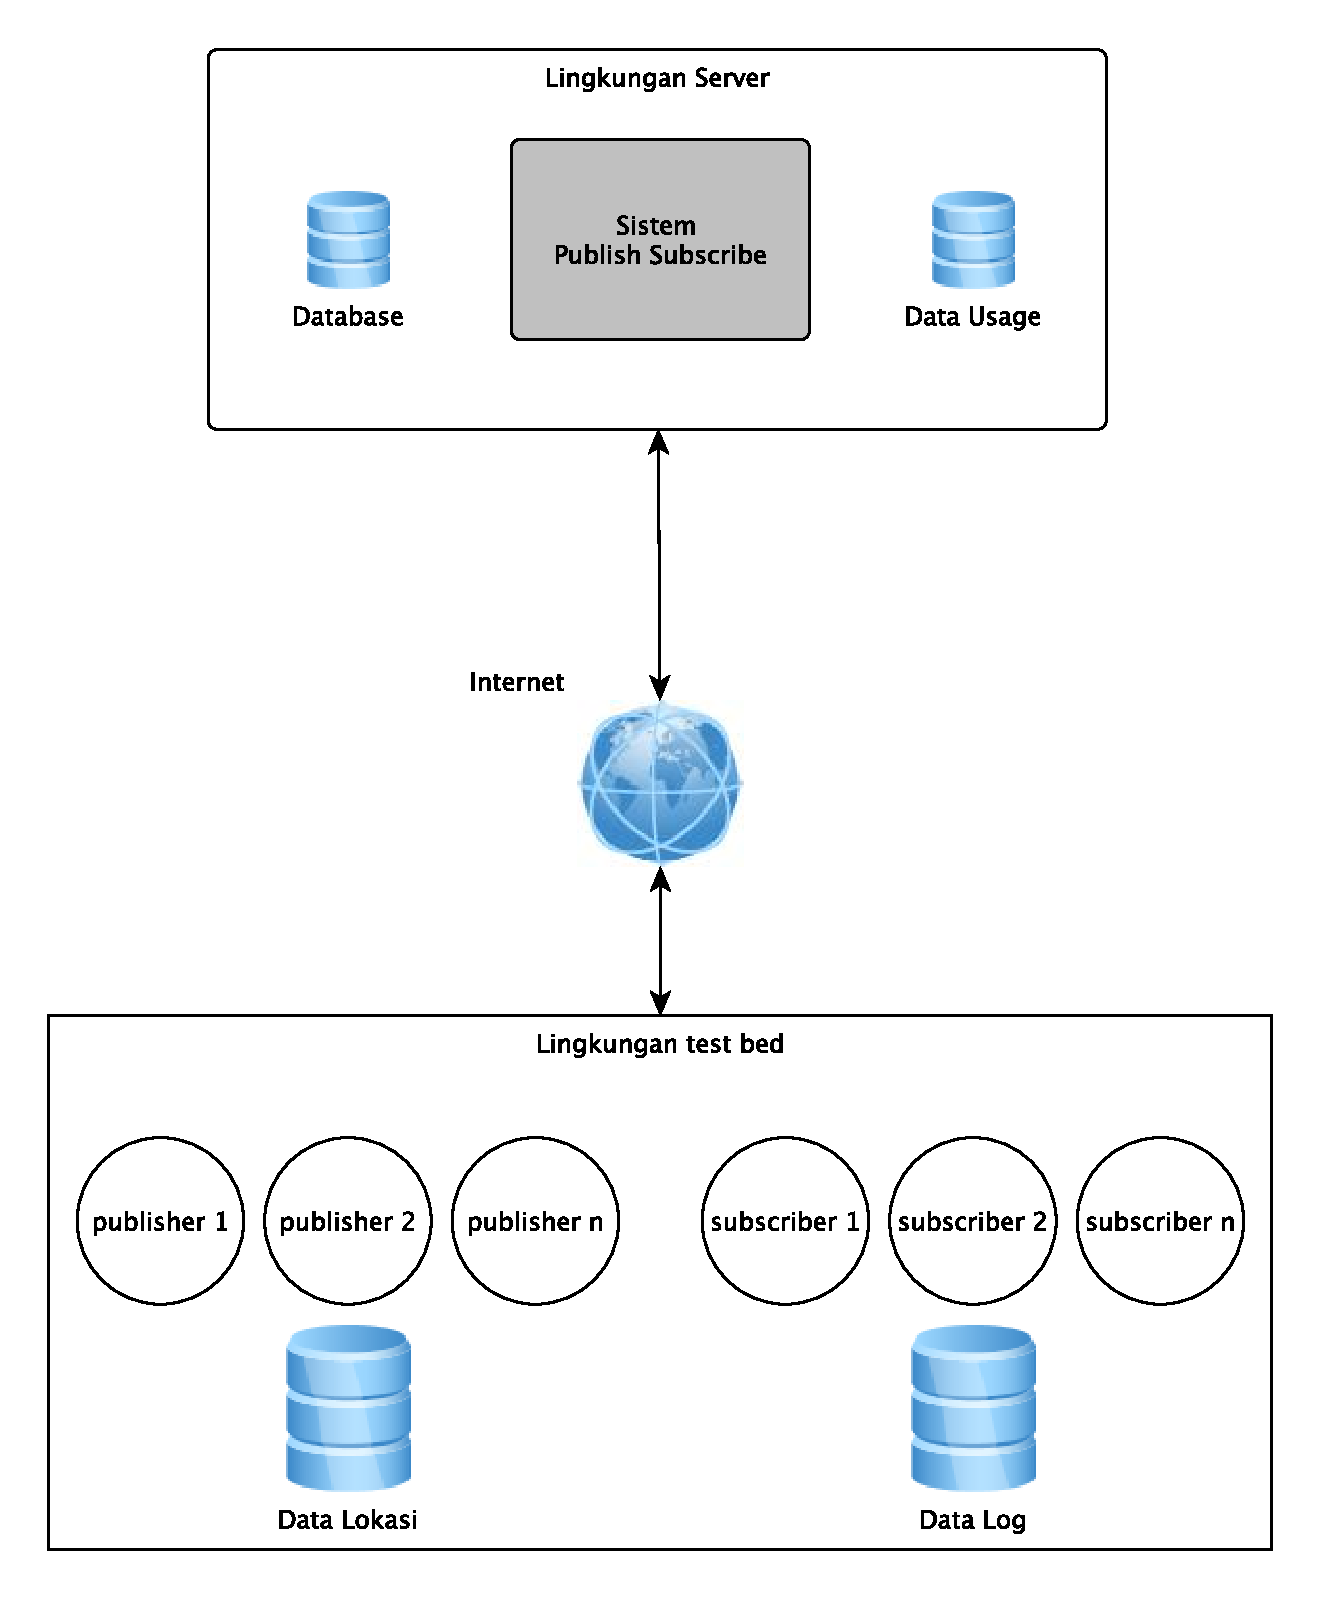
\includegraphics[scale=0.70]
	{images/4-testbed}
	\caption{Topologi \Testbed~Uji Coba}
\label{fig:testbed}
\end{figure}

% }}} Lingkungan Uji Coba %

% Skenario Pengujian {{{ %
\subsection{Skenario Pengujian}

Skenario pengujian pada penelitian ini dibagi menjadi empat bagian. Skenario
pengujian ini dilakukan untuk mengetahui kinerja \tracking~dengan model
interaksi \pubsub. Selain empat skenario pengujian tersebut, dalam proses uji
coba dilakukan pencatatan jumlah \event~\publish~yang terjadi. Hal ini bertujuan
untuk mengetahui pengaruh jumlah \publish~terhadap performa sistem yang
dirancang.

\begin{enumerate}
  [label=\alph*.
  ,noitemsep
  ,nolistsep
  ,leftmargin=0cm
  ,itemindent=.5cm
  ,listparindent=\parindent
  ]

	\item Uji coba penggunaan CPU \server
	\item Uji coba penggunaan RAM \server
  \item Uji coba \bandwidth
  \item Uji coba \latency

\end{enumerate}

% }}} Skenario Pengujian %

% Parameter Pengujian {{{ %
\subsection{Parameter Pengujian}

Sesuai dengan tujuan penelitian ini, yakni untuk membangun sistem
\tracking~multi target serta \f{update protocol} yang bersifat adaptif berbasis
\pubsub. Untuk mengetahui kualitas layanan, perlu adanya parameter-parameter
yang dapat mengidentifikasi perbaikan kualitas layanan model interaksi
\pubsub~adaptif.  Parameter-parameter yang digunakan dalam penelitian ini adalah
penggunaan CPU \server, penggunaan RAM \server, penggunaan \bandwidth, \latency.

\begin{enumerate}
  [label=\alph*.
  ,noitemsep
  ,nolistsep
  ,leftmargin=0cm
  ,itemindent=.5cm
  ,listparindent=\parindent
  ]

	\item Penggunaan CPU \Server

	Uji coba parameter penggunaan CPU dilakukan dengan mengukur penggunaan CPU
	ketika proses \tracking~dilakukan pada \broker. Uji coba akan dilakukan
	untuk setiap metode, yaitu non adaptif dan adaptif. Pengamatan uji coba
	dipengaruhi oleh jumlah \publisher~dan \subscriber. Uji coba dilakukan pada
  jaringan 3G dan jaringan Wi-Fi. Hasil dari masing-masing
	pengujian akan dibandingkan sehingga akan terlihat perbedaan penggunaan CPU
	pada proses \tracking~non adaptif maupun adaptif.

	\item Penggunaan RAM \Server

	Uji coba parameter memori dilakukan dengan mengukur penggunaan RAM ketika
	proses \tracking~dilakukan. Uji coba akan dilakukan untuk setiap metode, yaitu
	non adaptif dan adaptif. Pengamatan uji coba dipengaruhi oleh jumlah
	\publisher~dan \subscriber. Uji coba dilakukan pada jaringan 3G dan jaringan
  Wi-Fi. Hasil dari masing-masing pengujian akan
	dibandingkan sehingga akan terlihat perbedaan penggunaan RAM pada proses
	\tracking~non adaptif maupun adaptif.

	\item Penggunaan \bandwidth{}

  Uji coba parameter penggunaan \bandwidth~dilakukan dengan mengukur penggunaan
  \bandwidth~ketika terjadi interaksi antara \server~dan \client. Uji coba akan
  dilakukan sebanyak dua kali yakni menggunakan \f{update protocol} yang
  non-adaptif dan adaptif dengan model interaksi \pubsub. Uji coba dilakukan
  pada jaringan 3G dan jaringan Wi-Fi. Hasil dari
  masing-masing pengujian akan dibandingan sehingga akan terlihat perbedaan
  penggunaan \bandwidth~antara kedua uji coba.

  \item \Latency

	Uji coba parameter \latency~dilakukan dengan menghitung waktu antara
	\publish~konten paket informasi lokasi dikirimkan dari \publisher~ke
	\server~sampai diterima oleh \subscriber~berdasarkan dasar ketertarikan
	konten. Uji coba akan dilakukan sebanyak dua kali yakni menggunakan \f{update
		protocol} yang non-adaptif dan adaptif dengan model interaksi \pubsub. Uji
  coba dilakukan pada jaringan 3G dan jaringan Wi-Fi. Hasil
	dari masing-masing tiap pengujian akan dibandingkan untuk kemudian dapat
	dianalisa.

\end{enumerate}

% }}} Parameter Pengujian %

% }}} Uji Coba %

% Hasil Uji Coba dan Analisis {{{ %
\section{Hasil Uji Coba dan Analisis}

Pada penelitian ini, uji coba dilakukan dengan menggunakan lingkungan
\testbed~yang telah disiapkan. Paket informasi lokasi data sampel yang telah
diperoleh dimodifikasi dengan protokol tambahan sehingga proses
\event~\publish~hanya terjadi untuk paket informasi lokasi yang dibutuhkan saja.
Selain itu pada sisi \broker~disimpan informasi mengenai ketertarikan para
\subscriber~terhadap suatu informasi lokasi dari \publisher. Jika tidak ada
ketertarikan, maka \broker~memberikan notifikasi untuk menghentikan proses
\publish~informasi lokasi. Modifikasi ini dilakukan dengan tujuan untuk
menyediakan informasi lokasi yang hanya dibutuhkan pada kurun waktu tersebut.

Analisa data pada penelitian ini dilakukan dengan menguji fungsionalitas dari
\subscriber~yang berlaku sebagai \tracker. \Subscriber~dikatakan berfungsi
dengan baik apabila telah berjalan sesuai dengan rancangan sistem. Selain itu
analisa performa dilakukan juga untuk menguji \bandwidth, \latency, penggunaan
CPU serta penggunaan memori. Selain pemaparan hasil uji coba performa,
dijelaskan juga hasil uji fungsional sistem \tracking~multi target dengan
resolusi informasi lokasi.

% Hasil Uji Coba Performa {{{ %
\subsection{Hasil Uji Coba Performa}

Hasil uji coba performa disajikan untuk mengetahui bahwa performa \tracking~pada
lingkungan \pubsub~yang adaptif memiliki performa yang lebih baik.
Uji coba performa dilakukan dengan mengukur beberapa parameter pengujian yang
nantinya akan dibandingkan antara metode adaptif dengan non adaptif.
Parameter-parameter uji coba meliputi, penggunaan CPU \server, penggunaan RAM
\server, penggunaan \bandwidth~serta \latency. Selain itu dilakukan juga
pembandingan antara jumlah \event~\publish~pada metode adaptif dan metode
non-adaptif (\pubsub~tradisional).

% Jumlah Event Publish {{{ %
\subsubsection{Hasil Uji Coba Jumlah \Event~\Publish}

Hasil pengujian ini ditunjukkan untuk mengetahui pengaruh jumlah
\event~\publish~terhadap uji coba performa pada uji coba berikutnya. Pada
Tabel~\ref{tab:event_publish} ditunjukkan mengenai jumlah \event~\publish, baik
untuk metode adaptif maupun non-adaptif. Untuk metode non-adaptif, tidak ada
perbedaan \event-\publish~walaupun jumlah \subscriber~diubah. Simulasi uji coba
pada lingkungan \testbed~dilakukan selama 5 menit dengan interval jarak
\event~\publish~1 detik. Sehingga jumlah \event~\publish~pada metode non-adaptif
dapat dikalkulasikan dengan: jumlah publisher x 5 (merepresentasikan menit) x 60
(merepresentasikan detik).

\begin{table}
\centering
\caption{Jumlah \Event~\Publish}
\label{tab:event_publish}
\begin{tabular}{l l l l}
    \hline
    \Publisher & 5 \Subscriber~Adaptif  & 10 \Subscriber~Adaptif & Non-Adaptif \\
    \hline
    5  & 644 & 644  & 1500 \\
    10 & 712 & 1284 & 3000 \\
    15 & 794 & 1366 & 4500 \\
    20 & 864 & 1447 & 6000 \\
    25 & 945 & 1505 & 7500 \\
    \hline
  \end{tabular}
\end{table}

Sedangkan pada metode adaptif, jumlah \event~\publish~yang terjadi sangat
dipengaruhi oleh ada atau tidaknya ketertarikan konten informasi lokasi oleh
\subscriber. Semakin sedikit ketertarikan konten informasi, semakin sedikit pula
jumlah \event~\publish~yang terjadi. Walaupun jumlah \publisher~bertambah, tanpa
adanya perubahan ketertarikan konten, maka jumlah \event~\publish~tidak akan
berubah. Dapat dilihat jumlah \event~\publish~pada metode adaptif lebih kecil
jika dibandingan dengan metode non-adaptif. Diharapkan dengan adanya
pengurangan jumlah \event~\publish~dapat meningkatkan efisiensi performa pada
metode adaptif.

% }}} Jumlah Event Publish %

% Penggunaan CPU {{{ %
\subsubsection{Hasil Uji Coba Penggunaan CPU}

Hasil pengujian penggunaan CPU ditunjukkan untuk mengetahui berapakah rata-rata
penggunaan CPU pada proses \tracking~pada metode non-adaptif maupun adaptif.
Pengujian penggunaan CPU dilakukan sebanyak 10 kali untuk masing-masing metode,
baik metode adaptif maupun non-adaptif pada lingkungan \testbed.  Setiap
pengujian dilakukan perubahan jumlah \publisher~maupun \subscriber, baik
menggunakan jaringan 3G maupun jaringan Wi-Fi. Hasil uji coba penggunaan CPU
dengan metode adaptif menunjukkan bahwa rata-rata penggunaan CPU lebih kecil
seiring bertambahnya jumlah \publisher~dibandingkan dengan metode non-adaptif.

Pada jaringan 3G dengan jumlah 5 \subscriber, rata-rata penggunaan CPU sebesar
4,38 \% untuk metode adaptif. Sedangkan untuk metode non-adaptif, terjadi
peningkatan rata-rata penggunaan CPU menjadi 15,3 \%. Dengan peningkatan jumlah
\subscriber~sebesar 10, terjadi peningkatan rata-rata penggunaan CPU. Untuk
metode adaptif menjadi 6,74 \% dan metode non-adaptif menjadi 18,25 \%. Hasil
uji coba rata-rata penggunaan CPU untuk jaringan 3G ditunjukkan pada
Gambar~\ref{fig:3gcpu_5} dan Gambar~\ref{fig:3gcpu_10}.

\noindent
\begin{figure}
  \centering
  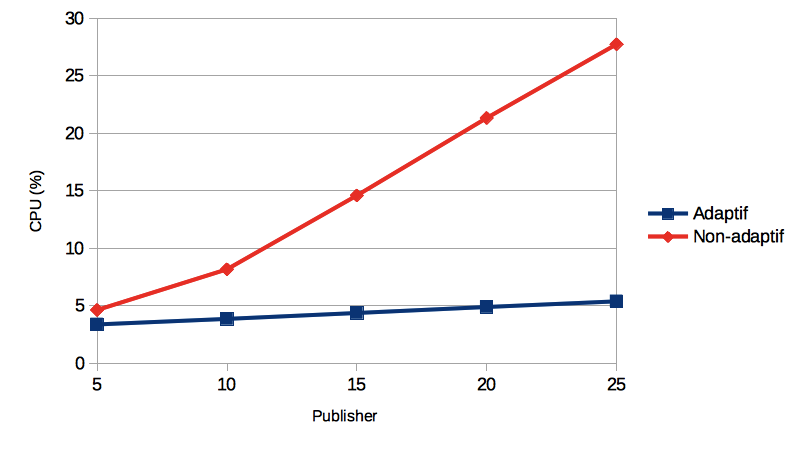
\includegraphics[scale=0.90]
	{images/4-3gcpu5.png}
	\caption{Hasil Uji Coba Penggunaan CPU 5 \Subscriber~dengan Jaringan 3G}
	\label{fig:3gcpu_5}
\end{figure}
\noindent

\begin{figure}
  \centering
  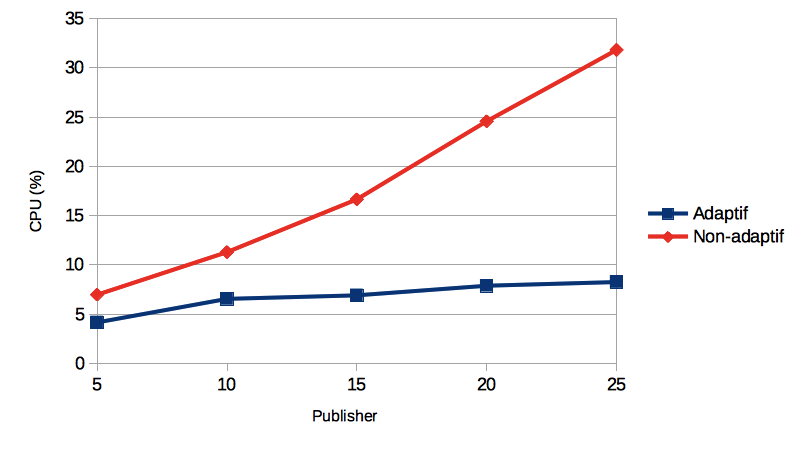
\includegraphics[scale=0.90]
	{images/4-3gcpu10.png}
	\caption{Hasil Uji Coba Penggunaan CPU 10 \Subscriber~dengan Jaringan 3G}
	\label{fig:3gcpu_10}
\end{figure}

Perilaku ini tak jauh berbeda dalam jaringan Wi-Fi. Rata-rata penggunaan CPU
untuk metode adaptif dengan jumlah 5 \subscriber, sebesar 4,92 \%. Sedangkan
untuk metode non-adaptif sebesar 13,99 \%. Ketika dilakukan perubahan jumlah
\subscriber, terjadi peningkatan untuk rata-rata penggunaan. Pada metode adaptif
dengan jumlah 10 \subscriber, rata-rata penggunaan CPU sebesar 7,51 \% sedangkan
untuk metode non-adaptif sebesar 17,68 \%. Hasil uji coba rata-rata penggunaan
CPU untuk jaringan Wi-Fi ditunjukkan pada Gambar~\ref{fig:cpu_5} dan
Gambar~\ref{fig:cpu_10}.

\noindent
\begin{figure}
  \centering
  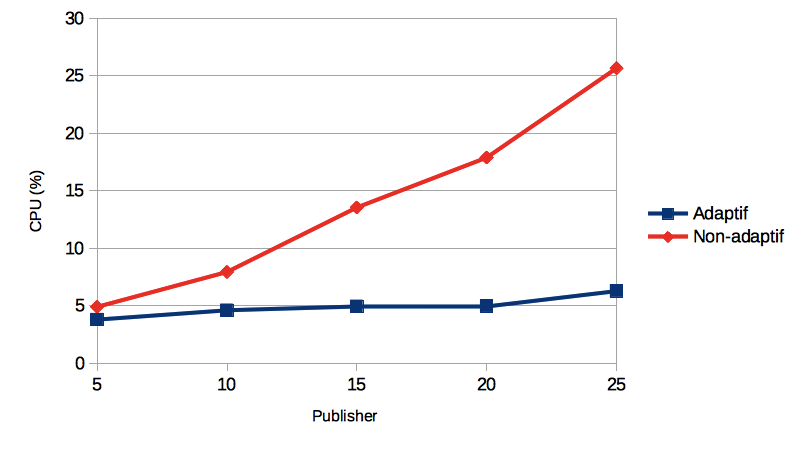
\includegraphics[scale=0.90]
	{images/4-cpu5.png}
	\caption{Hasil Uji Coba Penggunaan CPU 5 \Subscriber~dengan Jaringan Wi-Fi}
\label{fig:cpu_5}
\end{figure}
\noindent

\begin{figure}
  \centering
  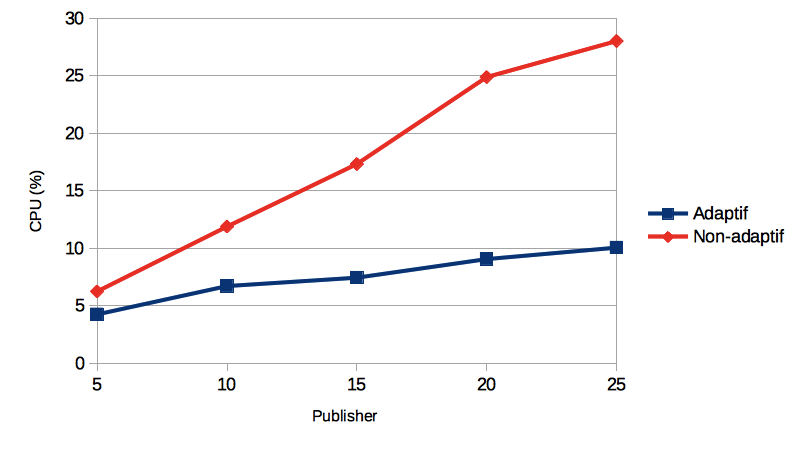
\includegraphics[scale=0.90]
	{images/4-cpu10.png}
	\caption{Hasil Uji Coba Penggunaan CPU 10 \Subscriber~dengan Jaingan Wi-Fi}
\label{fig:cpu_10}
\end{figure}

Dari dua skenario pengujian metode adaptif dan non-adaptif, dapat disimpulkan
bahwa rata-rata penggunaan CPU metode adaptif lebih baik, yakni lebih rendah
9-10 \% untuk uji coba dengan 5 \subscriber, dan 10-11 \% untuk uji coba dengan
10 \subscriber. Hal ini disebabkan karena semakin besar jumlah \publisher,
jumlah informasi lokasi yang harus dicocokkan ketertarikannya oleh \broker~akan
meningkat.  Pada metode adaptif proses pencocokkan tidak hanya dipengaruhi oleh
jumlah \publisher, tetapi pada kesesuaian ketertarikan informasi lokasi oleh
\subscriber. Informasi lokasi dari \publisher~yang sedang tidak diperlukan akan
dinotifikasi oleh \broker~untuk melakukan proses penghentian \publish. Proses
\publish~akan aktif kembali, jika informasi lokasi kembali dibutuhkan oleh
\subscriber.

% }}} Penggunaan CPU %

% Beban Memori {{{ %
\subsubsection{Hasil Uji Coba Beban RAM}

Hasil pengujian beban RAM ditunjukkan untuk mengetahui berapakah rata-rata
beban RAM pada proses \tracking~dengan metode adaptif dan non-adaptif. Pengujian
beban RAM dilakukan sebanyak 10 kali untuk masing-masing metode, dengan jumlah
\publisher~dan \subscriber~yang bervariasi. Pengujian akan dilakukan pada
jaringan 3G maupun jaringan Wi-Fi.

Hasil uji coba beban RAM menunjukkan bahwa rata-rata beban RAM untuk metode
non-adaptif cenderung lebih kecil dibandingkan dengan metode adaptif. Pada
jaringan 3G dengan 5 \subscriber~beban RAM metode non-adaptif sebesar
54783969,95 bytes dibandingkan metode adaptif sebesar 56898843,25 bytes. Untuk
10 \subscriber~beban RAM metode non-adaptif sebesar 56253726,15 bytes
dibandingkan metode adaptif sebesar 55474349,16 bytes. Grafik uji coba beban RAM
pada jaringan 3G ditunjukkan pada Gambar~\ref{fig:3gram_5} dan
Gambar~\ref{fig:3gram_10}.

\noindent
\begin{figure}
  \centering
  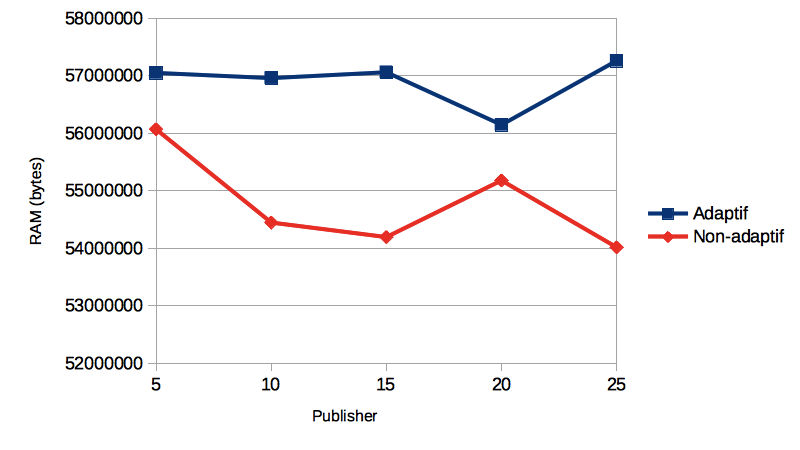
\includegraphics[scale=0.90]
	{images/4-3gram5.png}
	\caption{Hasil Uji Coba Beban RAM 5 \Subscriber~dengan Jaringan 3G}
\label{fig:3gram_5}
\end{figure}
\noindent

\begin{figure}
  \centering
  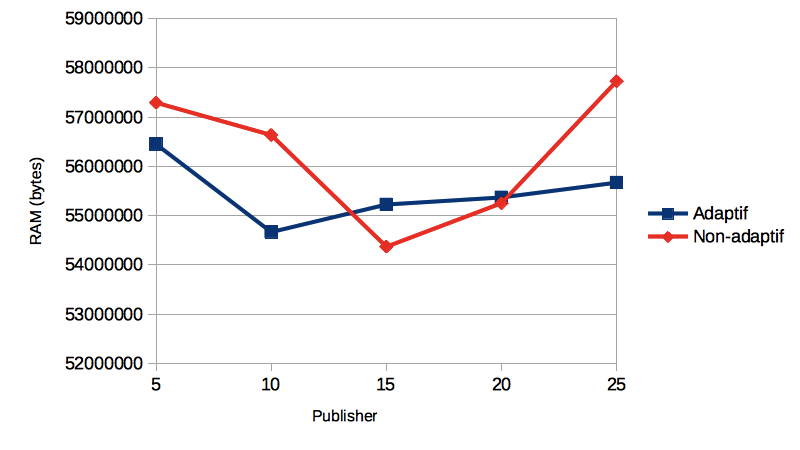
\includegraphics[scale=0.90]
	{images/4-3gram10.png}
	\caption{Hasil Uji Coba Beban RAM 10 \Subscriber~dengan Jaringan 3G}
	\label{fig:3gram_10}
\end{figure}

Pada jaringan Wi-Fi, rata-rata beban RAM untuk metode non-adaptif sebesar
54579197,96 bytes untuk 5 \subscriber. Lebih kecil dibandingkan dengan metode
adaptif sebesar 56818395,78 bytes. Jika dilakukan penambahan jumlah \subscriber
menjadi 10, perilaku ini tak jauh berbeda. Pada metode non-adaptif beban RAM
sebesar 54647938,67 bytes sedangkan untuk metode adaptif sebesar 55797926,39
bytes. Grafik uji coba beban RAM pada jaringan Wi-Fi ditunjukkan pada
Gambar~\ref{fig:ram_5} dan Gambar~\ref{fig:ram_10}.

\noindent
\begin{figure}
  \centering
  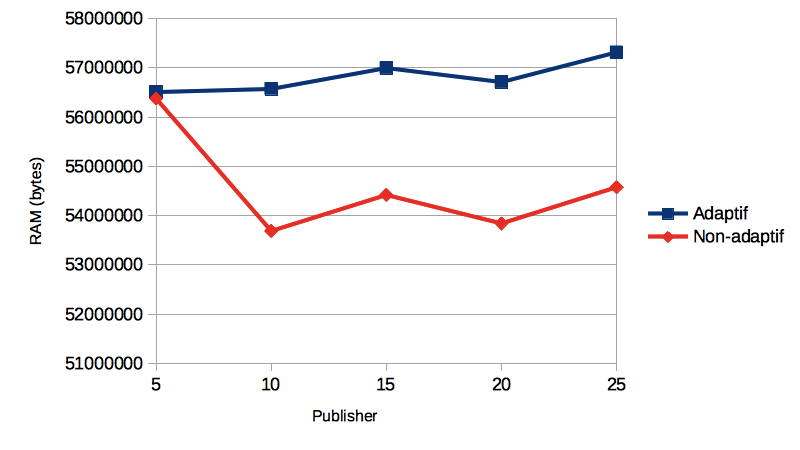
\includegraphics[scale=0.90]
	{images/4-ram5.png}
	\caption{Hasil Uji Coba Beban RAM 5 \Subscriber~dengan Jaringan Wi-Fi}
\label{fig:ram_5}
\end{figure}
\noindent

\begin{figure}
  \centering
  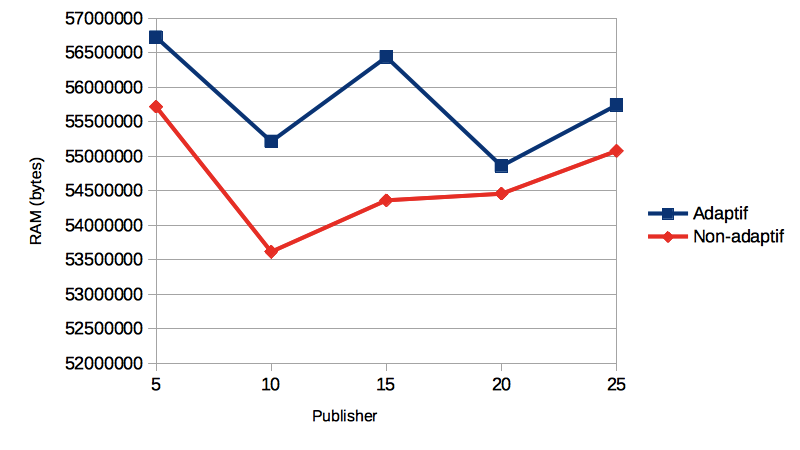
\includegraphics[scale=0.90]
	{images/4-ram10.png}
	\caption{Hasil Uji Coba Beban RAM 10 \Subscriber~dengan Jaringan Wi-Fi}
\label{fig:ram_10}
\end{figure}

Hal ini disebabkan dalam metode adaptif terdapat modul \idle~\manager~yang
bertugas untuk menjaga komunikasi hanya pada konten informasi lokasi yang
diperlukan. Konten-konten informasi yang dikirimkan oleh \publisher~akan
dilakukan pengecekan, jika informasi lokasi masih diperlukan proses pengiriman
lokasi akan dilanjutkan. Jika terjadi sebaliknya, \broker~akan memberikan
protokol kepada \publisher~untuk melakukan penghentian proses pengiriman untuk
sementara waktu. Pada selang waktu tertentu \broker~akan mengirimkan sebuah
protokol pengecekan untuk melakukan proses \publish~konten informasi lokasi atau
tidak. Sedangkan dalam metode non-adaptif, \publisher~akan melakukan
\publish~informasi lokasi setiap mendapat informasi yang baru.

% }}} Beban Memori %

% Penggunaan Bandwidth {{{ %
\subsubsection{Hasil Uji Coba Penggunaan \bandwidth}

Hasil pengujian \bandwidth~ditunjukkan untuk mengetahui berapakah besarnya
penggunaan \bandwidth~pada kedua metode, baik itu metode adaptif maupun
non-adaptif.  Untuk pengujian ini dilakukan sebanyak 10 kali untuk masing-masing
metode dengan jumlah \publisher~dan \subscriber~yang berbeda pada jaringan 3G
maupun jaringan Wi-Fi. Setiap pengujian dilakukan perubahan jumlah
\publiser~serta \subscriber.

\noindent
\begin{figure}
  \centering
  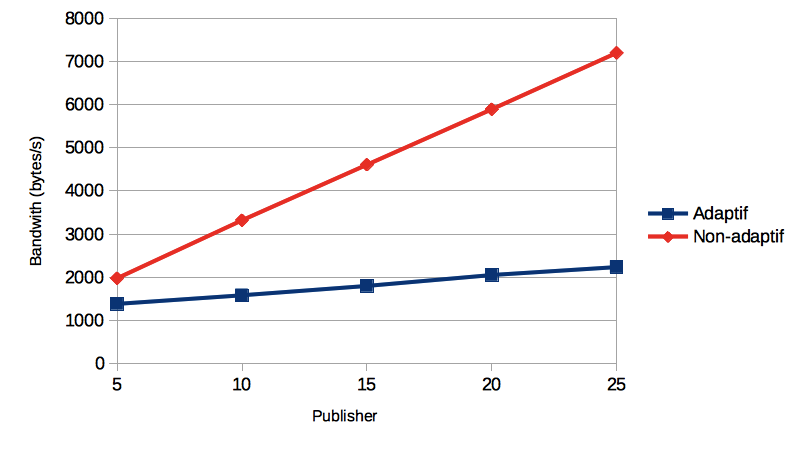
\includegraphics[scale=0.90]
	{images/4-3gbandwidth5.png}
	\caption{Hasil Uji Coba \Bandwidth~5 \Subscriber~dengan Jaringan 3G}
\label{fig:3gbandwidth_5}
\end{figure}
\noindent

\begin{figure}
  \centering
  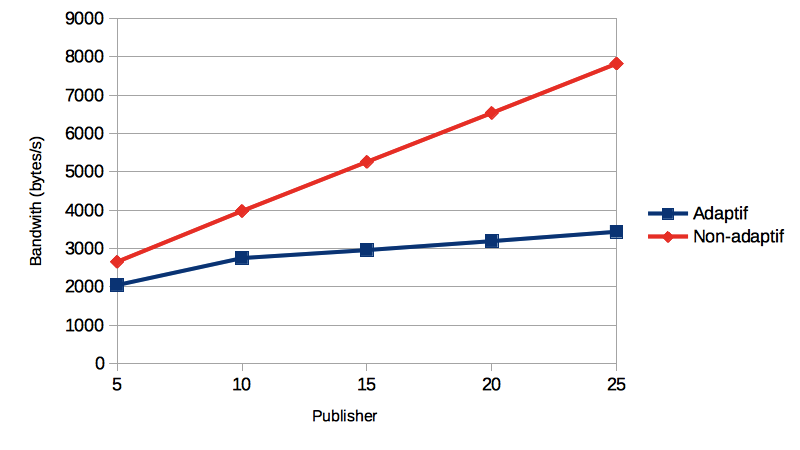
\includegraphics[scale=0.90]
	{images/4-3gbandwidth10.png}
	\caption{Hasil Uji Coba \Bandwidth~10 \Subscriber~dengan Jaringan 3G}
\label{fig:3gbandwidth_10}
\end{figure}

Hasil uji coba \bandwidth~pada jaringan 3G menunjukkan dari 10 kali percobaan
pada \tracking~metode adaptif lebih kecil rata-rata 2792,625 bytes/detik dari
\tracking~metode non-adaptif untuk 5 \subscriber~dengan rincian, adaptif
1805,975 bytes/detik dan non-adaptif 4598,6 bytes/detik. Untuk 10 \subscriber,
terjadi peningkatan pada penggunaan \bandwidth. Untuk metode adaptif menjadi
2873,634 bytes/detik dan metode non-adaptif sebesar 5246,973 bytes/detik. Hasil
uji coba penggunaan \bandwidth~pada jaringan 3G ditunjukkan pada
Gambar~\ref{fig:3gbandwidth_5} dan Gambar~\ref{fig:3gbandwidth_10}

\noindent
\begin{figure}
  \centering
  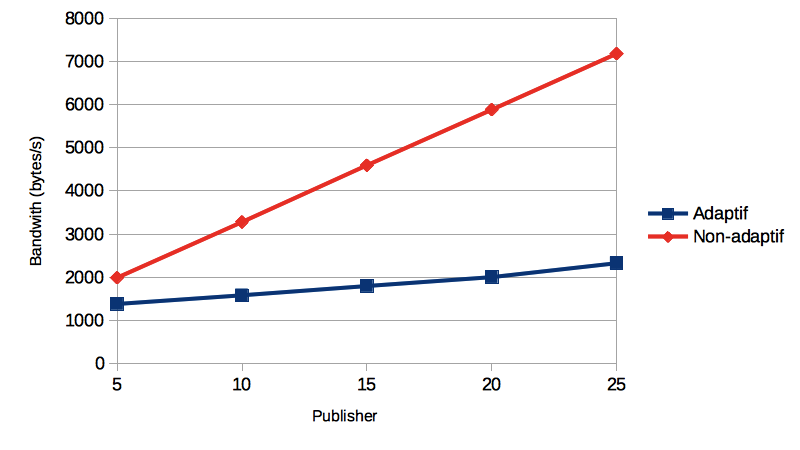
\includegraphics[scale=0.90]
	{images/4-bandwidth5.png}
	\caption{Hasil Uji Coba \Bandwidth~5 \Subscriber~dengan Jaringan Wi-Fi}
\label{fig:bandwidth_5}
\end{figure}
\noindent

\begin{figure}
  \centering
  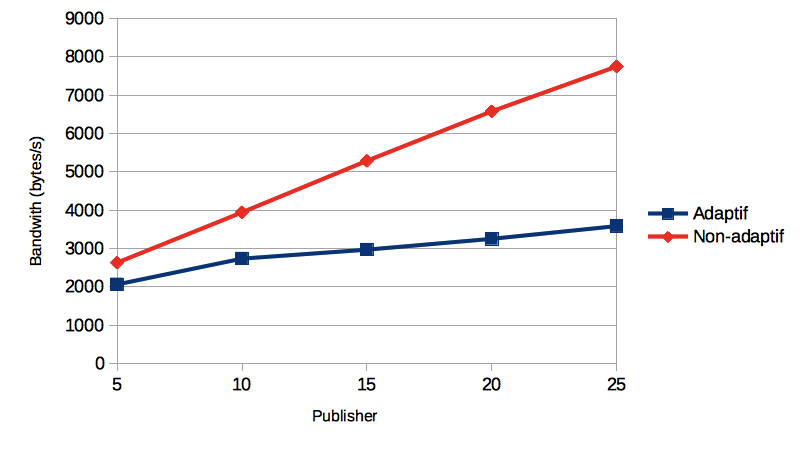
\includegraphics[scale=0.90]
	{images/4-bandwidth10.png}
	\caption{Hasil Uji Coba \Bandwidth~10 \Subscriber~dengan Jaringan Wi-Fi}
\label{fig:bandwidth_10}
\end{figure}

Pada jaringan Wi-Fi penggunaan \bandwidth~dengan 5 \subscriber~untuk metode
adaptif sebesar 1813,333 bytes/detik dan untuk metode non-adaptif sebesar
4584,952 bytes/detik. Dengan peningkatan jumlah \subscriber~terjadi peningkatan
penggunaan \bandwidth. Pada metode adaptif menjadi 2916,761 bytes/detik dan
metode non-adaptif 5234,661 bytes/detik. Grafik uji coba penggunaan
\bandwidth~pada jaringan Wi-Fi ditunjukkan pada Gambar~\ref{fig:bandwidth_5} dan
Gambar~\ref{fig:bandwidth_10}.

Hal ini disebabkan karena semakin besar jumlah \publisher~serta \subscriber,
maka lalu lintas jaringan akan semakin padat. Tetapi pada \tracking~metode
adaptif, selain hal ini dipengaruhi juga oleh ketertarikan informasi lokasi
\subscriber. Hanya informasi lokasi yang dibutuhkan oleh \subscriber~yang
disebarkan. Dengan demikian penggunaan \tracking~metode adaptif memberikan
dampak positif pada penggunaan \bandwidth~yang lebih baik dibandingan metode
non-adaptif.

% }}} Penggunaan Bandwidth %

% Latency {{{ %
\subsubsection{Hasil Uji Coba \Latency}

Hasil pengujian \latency~ditunjukkan untuk mengetahui berapakah rata-rata
\latency~antara kedua metode, adaptif dengan non-adaptif. Pengujian dilakukan
dengan jumlah \publisher~dan \subscriber~yang berbeda-beda pada jaringan 3G
maupun jaringan Wi-Fi. Proses ini dilakukan sebanyak 10 kali, untuk setiap metode.

Hasil uji coba menunjukkan adanya penurunan rata-rata \latency~untuk metode
adaptif dibandingkan dengan metode non-adaptif. Pada jaringan 3G dengan jumlah 5
\subscriber, rata-rata \latency~sebesar 309,821 ms untuk metode adaptif dan
542,789 ms untuk metode non-adaptif. Untuk 10 \subscriber, \latency~untuk metode
adaptif 204,98 ms dan 764,86 ms. Grafik hasil uji coba \latency~pada jaringan 3G
dapat dilihat pada Gambar~\ref{fig:3glatency_5} dan
Gambar~\ref{fig:3glatency_10}.

% Hasil uji coba \latency ditunjukkan pada
% Gambar~\ref{fig:latency_5} dan Gambar~\ref{fig:latency_10}.

\noindent
\begin{figure}
  \centering
  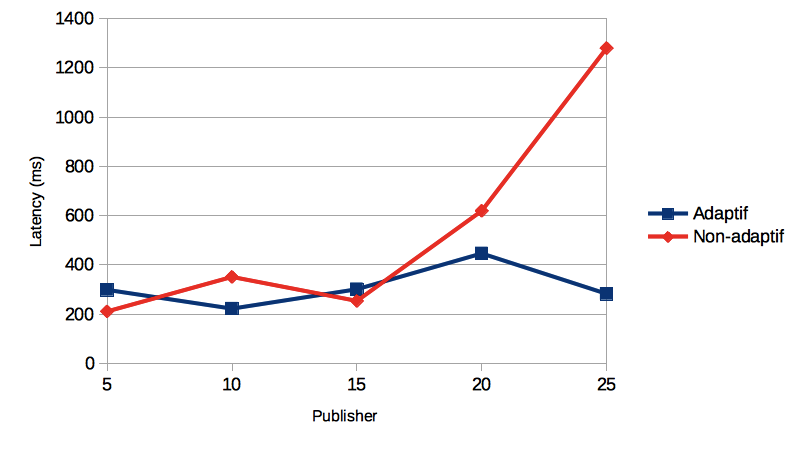
\includegraphics[scale=0.90]
	{images/4-3glatency5.png}
	\caption{Hasil Uji Coba \Latency~5 \Subscriber~dengan Jaringan 3G}
\label{fig:3glatency_5}
\end{figure}
\noindent

\begin{figure}
  \centering
  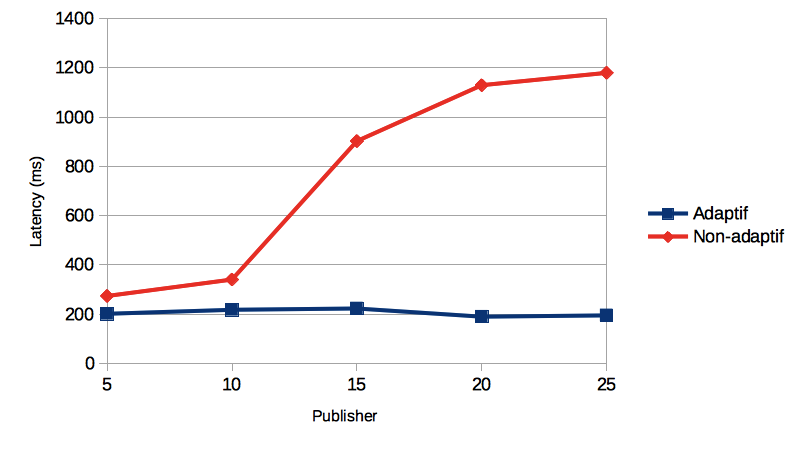
\includegraphics[scale=0.90]
	{images/4-3glatency10.png}
	\caption{Hasil Uji Coba \Latency~10 \Subscriber~dengan Jaringan 3G}
	\label{fig:3glatency_10}
\end{figure}

\noindent
\begin{figure}
  \centering
  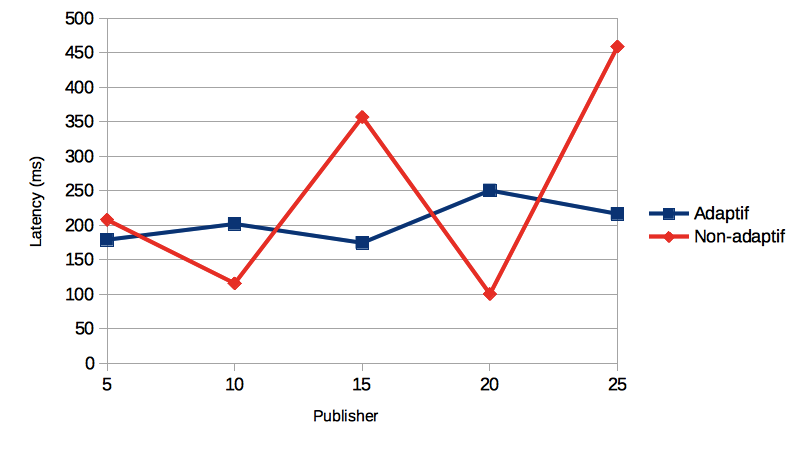
\includegraphics[scale=0.90]
	{images/4-latency5.png}
	\caption{Hasil Uji Coba \Latency~5 \Subscriber~dengan Jaringan Wi-Fi}
\label{fig:latency_5}
\end{figure}
\noindent

\begin{figure}
  \centering
  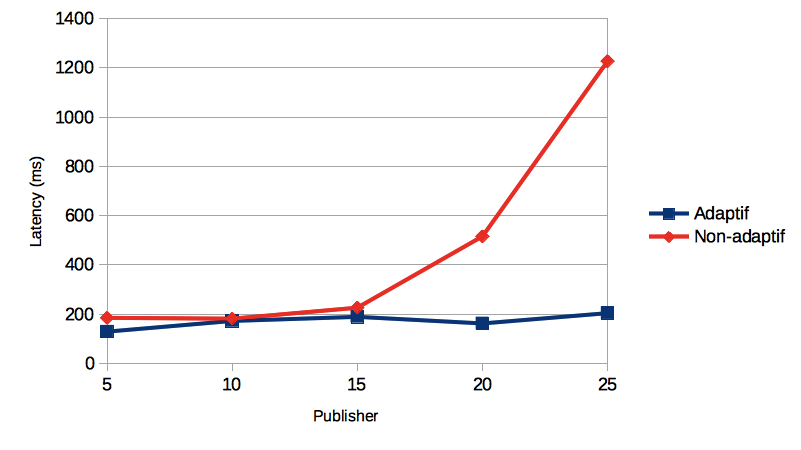
\includegraphics[scale=0.90]
	{images/4-latency10.png}
	\caption{Hasil Uji Coba \Latency~10 \Subscriber~dengan Jaringan Wi-Fi}
\label{fig:latency_10}
\end{figure}

Pada jaringan Wi-Fi, hasil uji coba \latency~menunjukkan rata-rata
\latency~untuk metode adaptif sebesar 204,644 ms lebih kecil dibandingkan
dengan non-adaptif sebesar 248,15 ms untuk 5 \subscriber. Untuk 10 subscriber,
metode adaptif sebesar 170,95 ms dan non-adaptif sebesar 466,78 ms. Rata-rata
\latency~pada jaringan Wi-Fi perbedaannya tidak terlalu besar jika dibandingkan
dengan jaringan 3G.

Penurunan \latency~pada metode adaptif disebabkan berkurangnya pengotor
informasi lokasi yang tidak diperlukan, dikarenakan tidak adanya ketertarikan
\subscriber~mengenai informasi tersebut. Pada proses \tracking~adaptif,
\publisher~hanya melakukan \publish~saat informasi itu benar-benar dibutuhkan.
Dengan demikian pengaplikasian metode adaptif dapat memberikan dampak positif
pada \tracking~dengan jumlah \publisher~yang banyak.

% }}} Latency %

% }}} Hasil Uji Coba Performa %

% Hasil Uji Coba Fungsional {{{ %
\subsection{Hasil Uji Coba Fungsionalitas}

Hasil uji coba fungsionalitas ini disajikan untuk mengetahui bahwa hasil yang
diperoleh sudah sesuai dengan sistem yang telah dirancang. Uji coba
fungsionalitas ini dilakukan pada proses mapping lokasi, \tracking~multi target
serta resolusi informasi lokasi.

% Fold description {{{ %
\subsubsection{Hasil Uji Coba Mapping Lokasi}

Mapping lokasi digunakan dalam penentuan resolusi informasi lokasi. Area
\tracking~yaitu Kampus Institut Sepuluh Nopember (ITS) telah dilakukan pembagian
wilayah sesuai dengan tingkat kedalaman resolusi informasi. Hal ini ditunjukkan
pada Gambar~\ref{fig:fungsional_area}. Sebagai contoh: dalam wilayah ITS dibagi
menjadi wilayah Zona FMIPA, Zona FTI. Dalam Zona FMIPA dibagi lagi menjadi
kedalaman resolusi yang lebih tinggi, yaitu: Gedung Jurusan Fisika, Gedung
Jurusan Statistika. Dengan adanya perbedaan resolusi informasi, informasi lokasi
dapat ditampilkan berbeda-beda tergantung dari tingkat kedalaman resolusi yang
diperlukan. Pada tingkat resolusi rendah, hanya didapatkan \centroid~lokasi dari
wilayah ITS. Untuk tingkat resolusi lebih tinggi didapatkan \centroid~lokasi
dari Zona FMIPA.

\noindent
\begin{figure}
  \centering
  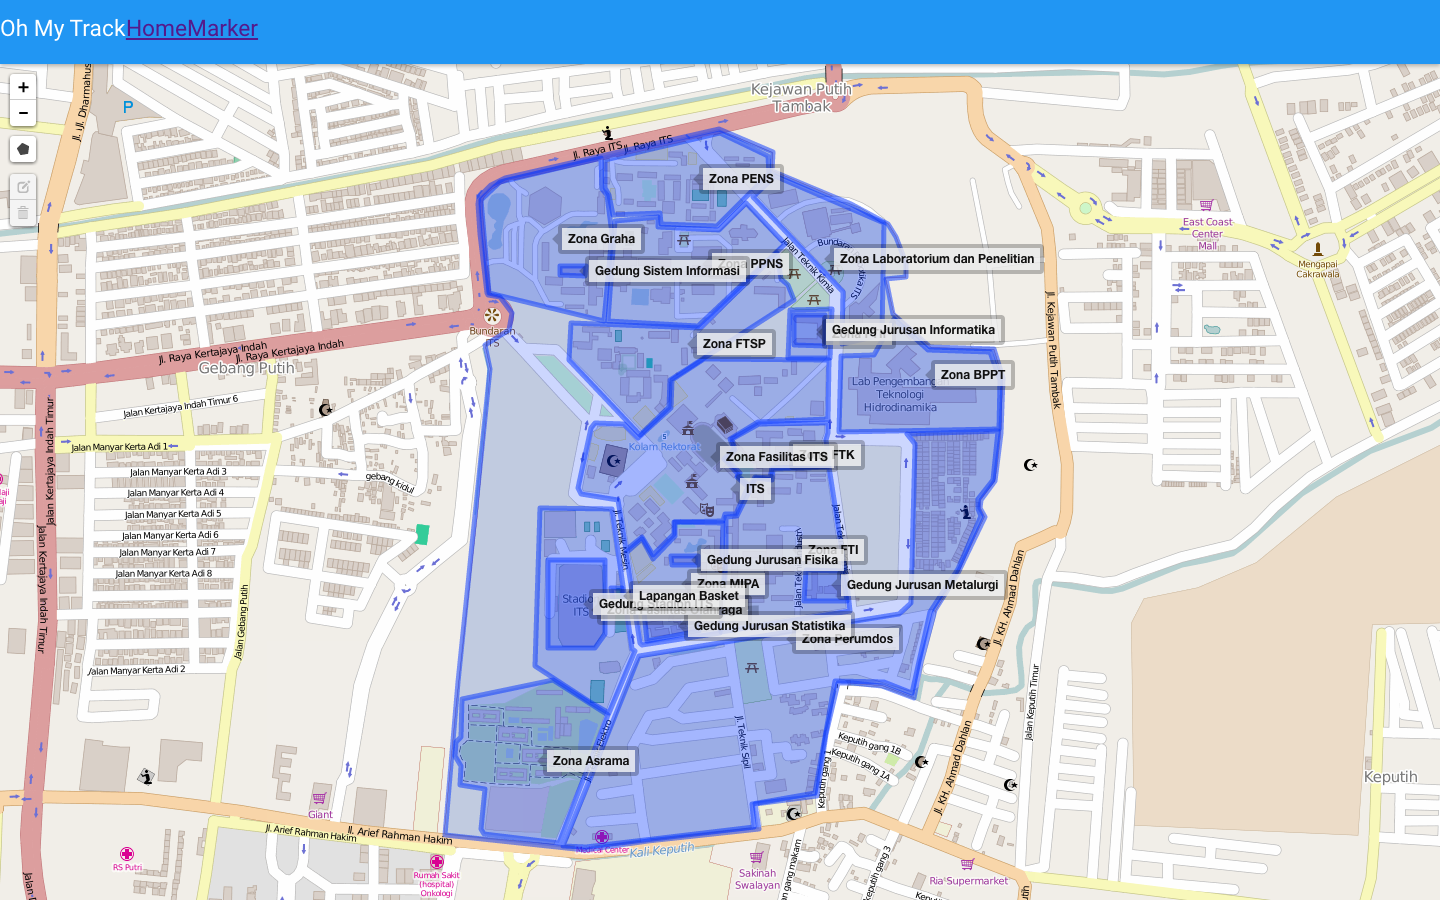
\includegraphics[scale=0.25]
	{images/4-fungsional-area.png}
  \caption{Uji Coba Fungsional Mapping Lokasi}
\label{fig:fungsional_area}
\end{figure}

% }}} Fold description %

% Hasil Uji Coba Tracking Multi Target {{{ %
\subsubsection{Hasil Uji Coba \Tracking~Multi Target}

Hasil uji coba ini ditunjukkan untuk mengetahui kemampuan sistem \tracking~untuk
menerima informasi lokasi berdasarkan ketertarikan \subscriber. Pada
Gambar~\ref{fig:fungsional_multi} dapat dilihat dua marker yang berwarna merah
dan biru pada wilayah \tracking~yang didasarkan pada ketertarikan \subscriber.
Kemampuan ini berlaku juga untuk sebaliknya, seorang \publisher~dapat
di-\track~oleh lebih dari satu \subscriber. Hal ini dapat dilihat pada
Gambar~\ref{fig:fungsional_resolusi}.

\Subscriber~mempunyai ketertarikan konten informasi berupa semua \publisher~yang
berada dalam area Kampus ITS yang dinotasikan dalam \f{area = ITS}. Semua
\publisher~yang melakukan \publish~informasi lokasi dalam area Kampus ITS akan
ditampilkan. Ketika terdapat \publisher~baru yang \publish~informasi lokasi yang
sesuai dengan ketertarikan, akan ditampilkan tanpa merubah konten ketertarikan.

\noindent
\begin{figure}
  \centering
  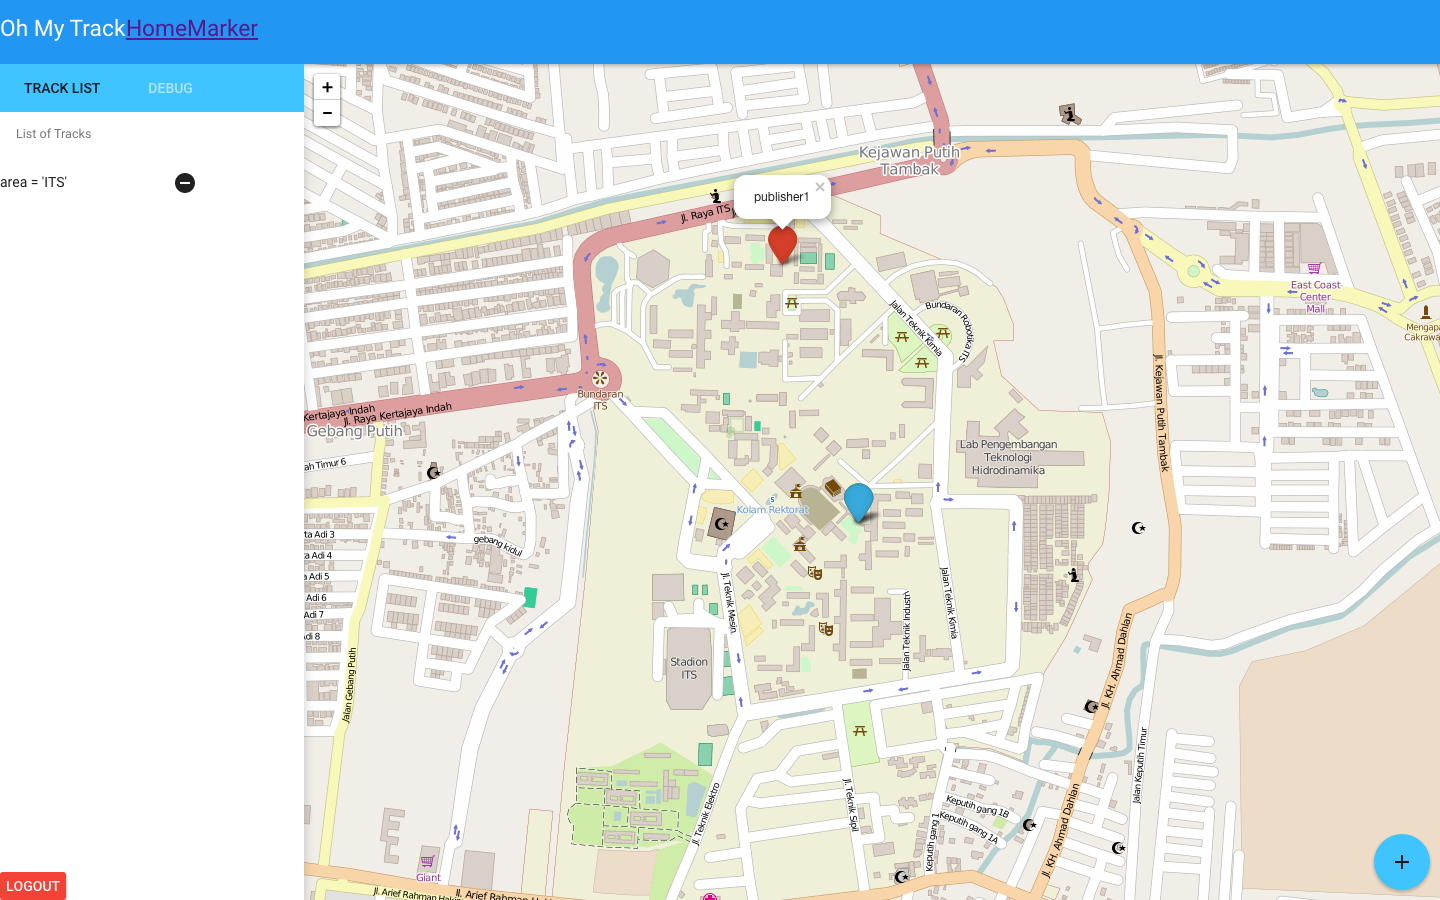
\includegraphics[scale=0.25]
	{images/4-fungsional-multi.png}
  \caption{Uji Coba Fungsional Multi Target}
\label{fig:fungsional_multi}
\end{figure}

% }}} Hasil Uji Coba Tracking Multi Target %

% Hasil Uji Coba Resolusi {{{ %
\subsubsection{Hasil Uji Coba Resolusi Informasi Lokasi}

Hasil uji coba resolusi ditunjukkan untuk mengetahui keberhasilan sistem
\tracking~untuk menyembunyikan informasi lokasi berdasarkan level hak akses.
Pada Gambar~\ref{fig:fungsional_resolusi} ditunjukkan dua \subscriber~yang
mempunyai level hak akses berbeda, yaitu koordinat dan area. Informasi lokasi
koordinat diwakili dengan simbol warna merah, sedangkan untuk area berwarna
hitam. Dari Gambar~\ref{fig:fungsional_resolusi} dapat dilihat perbedaan
informasi lokasi yang berbeda untuk \publisher~yang sama.

\noindent
\begin{figure}
  \centering
  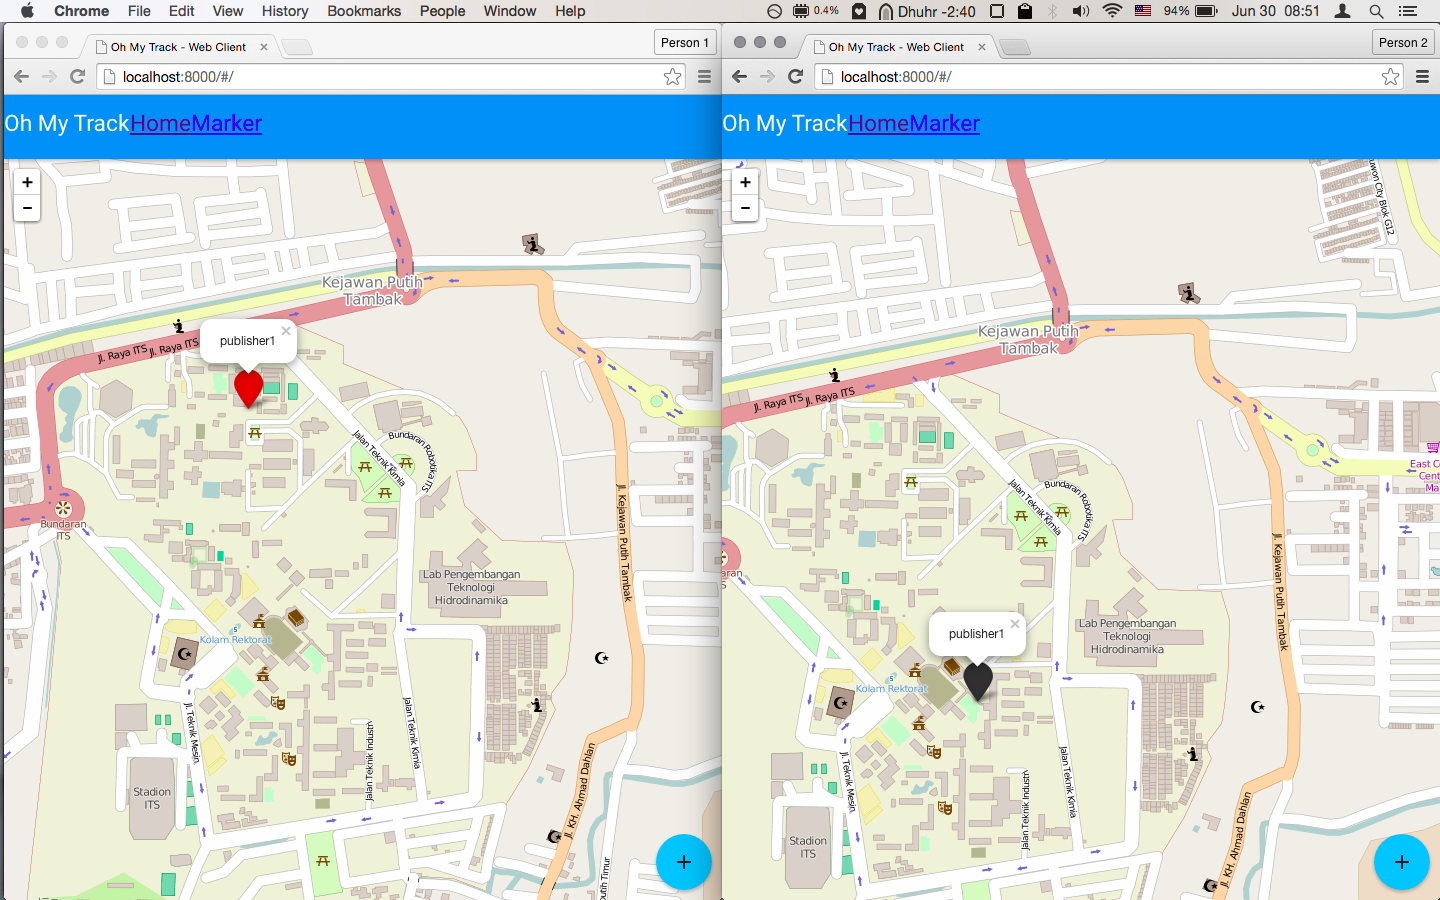
\includegraphics[scale=0.25]
	{images/4-fungsional-resolusi.png}
  \caption{Uji Coba Fungsional Resolusi}
\label{fig:fungsional_resolusi}
\end{figure}

\Subscriber~dengan level hak akses koordinat akan mendapatkan informasi lokasi
serupa dengan informasi lokasi yang di-\publish~oleh \publisher. Informasi paket
lokasi yang di-\publish~dipaparkan paga Gambar~\ref{fig:publisher1}. Sedangkan
informasi paket lokasi dengan level hak akses koordinat dapat dilihat pada
Gambar~\ref{fig:subscriber1}. Sedangkan \subscriber~dengan level hak akses area
hanya akan mendapatkan informasi lokasi berupa \centroid~area level hak akses
terdekat. Informasi paket lokasi dengan level hak akses area dapat dilihat pada
Gambar~\ref{fig:subscriber4}.

\begin{figure}
	\centering
	\lstset{basicstyle=\ttfamily,frame=single,language=javascript}
	\lstinputlisting{src/publisher1.json}
	\caption{Informasi Paket Lokasi \Publisher}
\label{fig:publisher1}
\end{figure}

Pada Gambar~\ref{fig:subscriber1} dan Gambar~\ref{fig:subscriber4} dapat dilihat
adanya perbedaan nilai atribut level. Nilai ini menjadi acuan pada sistem
\pubsub~untuk menyembunyikan informasi sebelum dikirimkan kepada
\subscriber~yang mempunyai ketertarikan.

\noindent
\begin{figure}
	\centering
	\lstset{basicstyle=\ttfamily,frame=single,language=javascript}
	\lstinputlisting{src/subscriber1.json}
	\caption{Informasi Paket dengan Resolusi Level Koordinat}
\label{fig:subscriber1}
\end{figure}

\noindent
\begin{figure}
	\centering
	\lstset{basicstyle=\ttfamily,frame=single,language=javascript}
	\lstinputlisting{src/subscriber4.json}
	\caption{Informasi Paket dengan Resolusi Level Area}
\label{fig:subscriber4}
\end{figure}

% }}} Hasil Uji Coba Resolusi %

% }}} Hasil Uji Coba Fungsional %

% }}} Hasil Uji Coba dan Analisis %
